%!TEX TS-program=xelatex
\documentclass[xetex]{beamer}

\usefonttheme{professionalfonts}
\usepackage[UTF8]{ctex}
\usepackage{hyperref}
\usepackage{unicode-math}
\usepackage{amsmath, amssymb}
\usepackage{graphicx, wrapfig}
\usepackage{nopageno}

\DeclareMathOperator{\argmax}{argmax}

\usetheme[block=fill, subsectionpage=progressbar]{metropolis}

\setmathfont{XITS Math}

%这是标题页
\title{重积分}
\subtitle{重积分的变量代换}
\author{数学分析MOOC小组 }
%这是标题页

\begin{document}

\frame{\maketitle}

\begin{frame}
    \frametitle{回顾:定积分的变量代换}
    若$f(x)$在$[a,b]$连续,变量代换$x=\varphi(t)$在$\alpha\leq t \leq\beta$可微$,\varphi(\alpha)=a,\varphi(\beta)=b$,则
    $$\int_a^bf(x)dx=\int_{\alpha}^{\beta}f(\varphi(t))\varphi^{'}(t)dt.$$
\end{frame}

\begin{frame}
    \frametitle{一种导数表示}
    有变量代换
    $$\begin{cases}
        x=\varphi(u,v),\\
        y=\psi(u,v)
    \end{cases}$$
    则有,
    $$J(u,v)=\dfrac{\partial(x,y)}{\partial(u,v)}=\left|
        \begin{matrix}
             \dfrac{\partial\varphi}{\partial u} & \dfrac{\partial \varphi}{\partial v} \\\\
             \dfrac{\partial\psi}{\partial u} & \dfrac{\partial \psi}{\partial v}
         \end{matrix}
         \right|$$
\end{frame}

\begin{frame}
    \frametitle{重积分变量代换定理}
    设变换$T:$
    $$\begin{cases}
        x=\varphi(u,v),\\
        y=\psi(u,v)
    \end{cases}$$
    把$Ouv$平面上由逐段光滑的闭曲线围成的区域$\Delta$一一映射为$Oxy$平面的区域$D$,且$\varphi,\psi$在$\Delta$有二阶连续偏导数,
    \begin{center}
    $J(u,v)=\dfrac{\partial(x,y)}{\partial(u,v)}\neq0$ \quad 当$(u,v)\in\Delta,$
    \end{center}
    而$f(x,y)$是定义在$D$上的连续函数,则
    $$\iint\limits_Df(x,y)dxdy=\iint\limits_{\Delta}f(\varphi(u,v),\psi(u,v)) | J(u,v)|dudv.$$
\end{frame}

\begin{frame}
    \frametitle{极坐标代换}
    做变换
    $$\begin{cases}
        x=r\cos{\theta},\\
        y=r\sin{\theta}
    \end{cases}$$
    变换的函数行列式为
    $$\dfrac{\partial(x,y)}{\partial(r,\theta)}=
    \begin{vmatrix}
        \cos{\theta} & -r\sin{\theta} \\
        \sin{\theta} & r\cos{\theta}
    \end{vmatrix}
    =r.$$
    计算公式
    $$\iint\limits_Df(x,y)dxdy=\iint\limits_{\Delta}f(r\cos{\theta},r\sin{\theta})rdrd\theta.$$
\end{frame}

\begin{frame}
    \frametitle{极坐标代换例题}
    \begin{figure}[ht]
        \centering %图片居中放置
        % 在这里使用 \includegraphics 插入图片,改变width就可以改变图片的大小。
       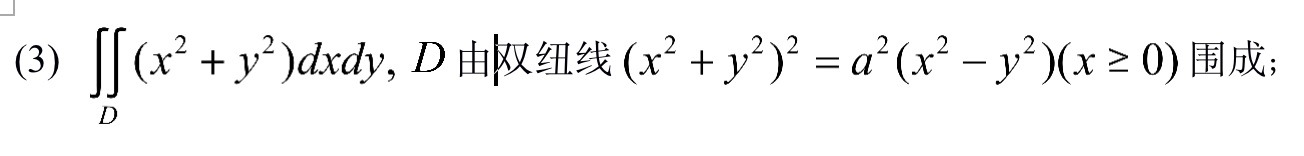
\includegraphics[width=1.0\textwidth]{img/a.jpg}
    \end{figure}
    \pause
    做变换
    $$\begin{cases}
        x=r\cos{\theta},\\
        y=r\sin{\theta}
    \end{cases}$$
    原函数变为
    $$r = a \sqrt{\cos{2 \theta}} $$
    $$- \frac{\pi}{4} < \theta < \frac{\pi}{4}, \quad 0 \leq r \leq a \sqrt{\cos{2 \theta}} $$
\end{frame}
    
\begin{frame}
    \frametitle{极坐标代换例题}
    \begin{figure}[ht]
        \centering %图片居中放置
        % 在这里使用 \includegraphics 插入图片,改变width就可以改变图片的大小。
       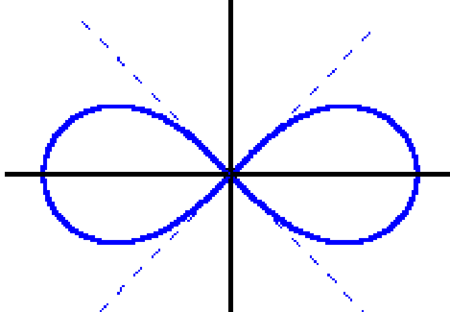
\includegraphics[width=0.5\textwidth]{img/c.jpg}
    \end{figure}
    \pause
    解:
    \begin{align*} 
        \iint \limits_D (x^2 + y^2) dxdy &= \int _{ - \frac{4}{\pi} } ^{ \frac{4}{\pi} } d \theta \int _0 ^{a \sqrt{ \cos{2 \theta} } } r^3 dr = \frac{a^2} {4} \int  _{ - \frac{4}{\pi} } ^{ \frac{4}{\pi} } \cos ^2 {2 \theta} d \theta \\
        &= \frac {a^2} {8} \int _{ - \frac{4}{\pi} } ^{ \frac{4}{\pi} } (1+ \cos{4 \theta}) d \theta = \frac{\pi} {16} a^2
    \end{align*}
\end{frame}

\begin{frame}
    \frametitle{极坐标代换例题}
    求椭球体的体积$V$,椭球体为
    $$\dfrac{x^2}{a^2}+\dfrac{y^2}{b^2}+\dfrac{z^2}{c^2}\leq1$$
    \pause
    由对称性知,
    $$V=2\iint\limits_Dc\sqrt{1-\frac{x^2}{a^2}-\frac{y^2}{b^2}}dxdy,$$
    \begin{center}
    其中$D=\left\{(x,y) \left| \dfrac{x^2}{a^2}+\dfrac{y^2}{b^2}\leq1\right\}.$
    \end{center}
\end{frame}    

\begin{frame}
    \frametitle{极坐标代换例题}
    做广义极坐标变换
    $$x=ar\cos{\theta}, y=br\sin{\theta}$$
    则$D$对应于$0\leq r \leq1, 0\leq\theta\leq2\pi.$而
    $$J(r,\theta)=\dfrac{\partial (x,y)}{\partial (r,\theta)}=\left|
        \begin{matrix}
             a\cos{\theta} & -ar\sin{\theta} \\
             b\sin{\theta} & br\cos{\theta}
         \end{matrix}
         \right|=abr$$
\end{frame}  

\begin{frame}
    \frametitle{极坐标代换例题}
    因此
    \begin{align*}
    V &= 2\int _0 ^{2 \pi} d \theta \int _0^1 c \sqrt{1 - r^2} abrdr\\
      &=4 \pi abc \int _0 ^1 \sqrt{1 - r^2} rdr \quad = \quad 4 \pi abc \frac{1}{2} \cdot \frac{2}{3} (1 - r^2) ^{\frac{3}{2}} \Big\vert _1 ^0 \\
      &= \frac{4}{3} \pi abc.
     \end{align*}
\end{frame} 

\begin{frame}
    \frametitle{三重积分的变量代换}
    做变换
    $$\begin{cases}
         x=x(u,v,w) \\
         y=y(u,v,w) \\
           z=z(u,v,w)
    \end{cases} $$   
    则
    \begin{align*}
    &\iiint\limits_V f(x,y,z) dxdydz \\
    = &\iiint\limits_\Omega f(x(u,v,w), y(u,v,w), z(u,v,w)) \left| \dfrac{\partial (x,y,z)}{\partial (u,v,w)} \right| dudvdw
    \end{align*}
\end{frame} 

\begin{frame}
    \frametitle{柱坐标代换}
    变换
    $$\begin{cases}
        x=r \cos{\theta}, \qquad 0 \leq r < + \infty, \\
        y=r \sin{\theta}, \qquad 0 \leq  \theta < 2 \pi \\
        z=z, \qquad \qquad - \infty < z < + \infty
    \end{cases}$$
    这时
    $$J(r , \theta , z) = \dfrac{\partial (x,y,z)}{\partial (r, \theta ,z)} = \left|
    \begin{matrix}
        \cos{\theta} & -r\sin{\theta} & 0 \\
        \sin{\theta} & r\cos{\theta} & 0 \\
        0  & 0 & 1
    \end{matrix} \right| = r$$
    PS:$z$不变,$x,y$变为对应的极坐标。
\end{frame} 

\begin{frame}
    \frametitle{柱坐标代换}
    因此变量代换公式为
    $$\iiint \limits_V f(x,y,z) dxdydz =  \iiint \limits_{\Omega} f(r \cos{\theta} , r \sin{\theta} , z) rdrd \theta dz. $$
\end{frame} 

\begin{frame}
    \frametitle{球坐标代换}
    做变换
    $$\begin{cases}
        x = r \cos{\theta} \sin{\varphi} , \quad 0 \leq r < + \infty \\
        y = r \sin{\theta} \sin{\varphi} , \quad 0 \leq \theta < 2 \pi \\
        z = r \cos{\varphi} , \qquad \quad 0 \leq \varphi \leq \pi \\
    \end{cases}$$
    PS:$\theta$代表经度,$\varphi$代表维度,$r$代表与地心的距离。\\
    \begin{figure}[ht]
        \centering %图片居中放置
        % 在这里使用 \includegraphics 插入图片,改变width就可以改变图片的大小。
       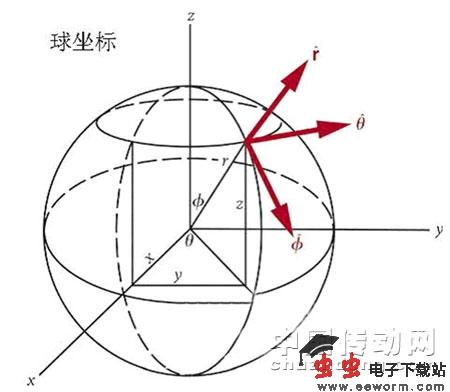
\includegraphics[width=0.4\textwidth]{img/g.jpg}
    \end{figure}
\end{frame} 

\begin{frame}
    \frametitle{球坐标代换}
    这时
    \begin{align*}
         &J(r , \theta , \varphi) = \dfrac {\partial (x,y,z)} {\partial (r, \theta , \varphi)} \\
         =&\left|
         \begin{matrix}
             \cos{\theta} \sin{\varphi} & -r \sin{\theta} \sin{\varphi} & r \cos{\theta} \cos{\varphi} \\
             \sin{\theta} \sin{\varphi} & r \cos{\theta} \sin{\varphi} & r \sin{\theta} \cos{\varphi} \\
             \cos{\varphi} & 0 & -r \sin{\varphi} 
         \end{matrix} \right| = - r^2 \sin{\varphi},
    \end{align*} 
     因此变量代换公式为
    \begin{align*}
        &\iiint \limits_V f(x,y,z) dxdydz \\
        =  &\iiint \limits_{\Omega} f(r \cos{\theta} \sin{\varphi} , r \sin{\theta} \sin{\varphi} , r \cos{\varphi}) r^2        \sin{\varphi} drd \theta d \varphi . 
    \end{align*}
\end{frame} 

\begin{frame}
    \frametitle{三重坐标代换例题}
    \begin{figure}[ht]
        \centering %图片居中放置
        % 在这里使用 \includegraphics 插入图片,改变width就可以改变图片的大小。
       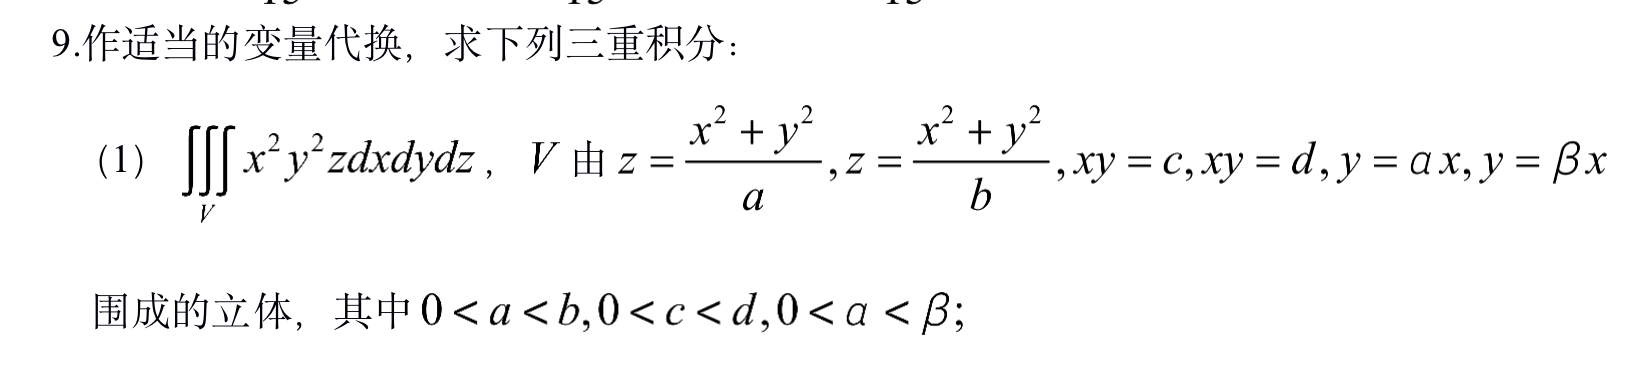
\includegraphics[width=1.0\textwidth]{img/e.jpg}
    \end{figure}
\end{frame} 

\begin{frame}
    \frametitle{三重坐标代换例题}
    \begin{figure}[ht]
        \centering %图片居中放置
        % 在这里使用 \includegraphics 插入图片,改变width就可以改变图片的大小。
       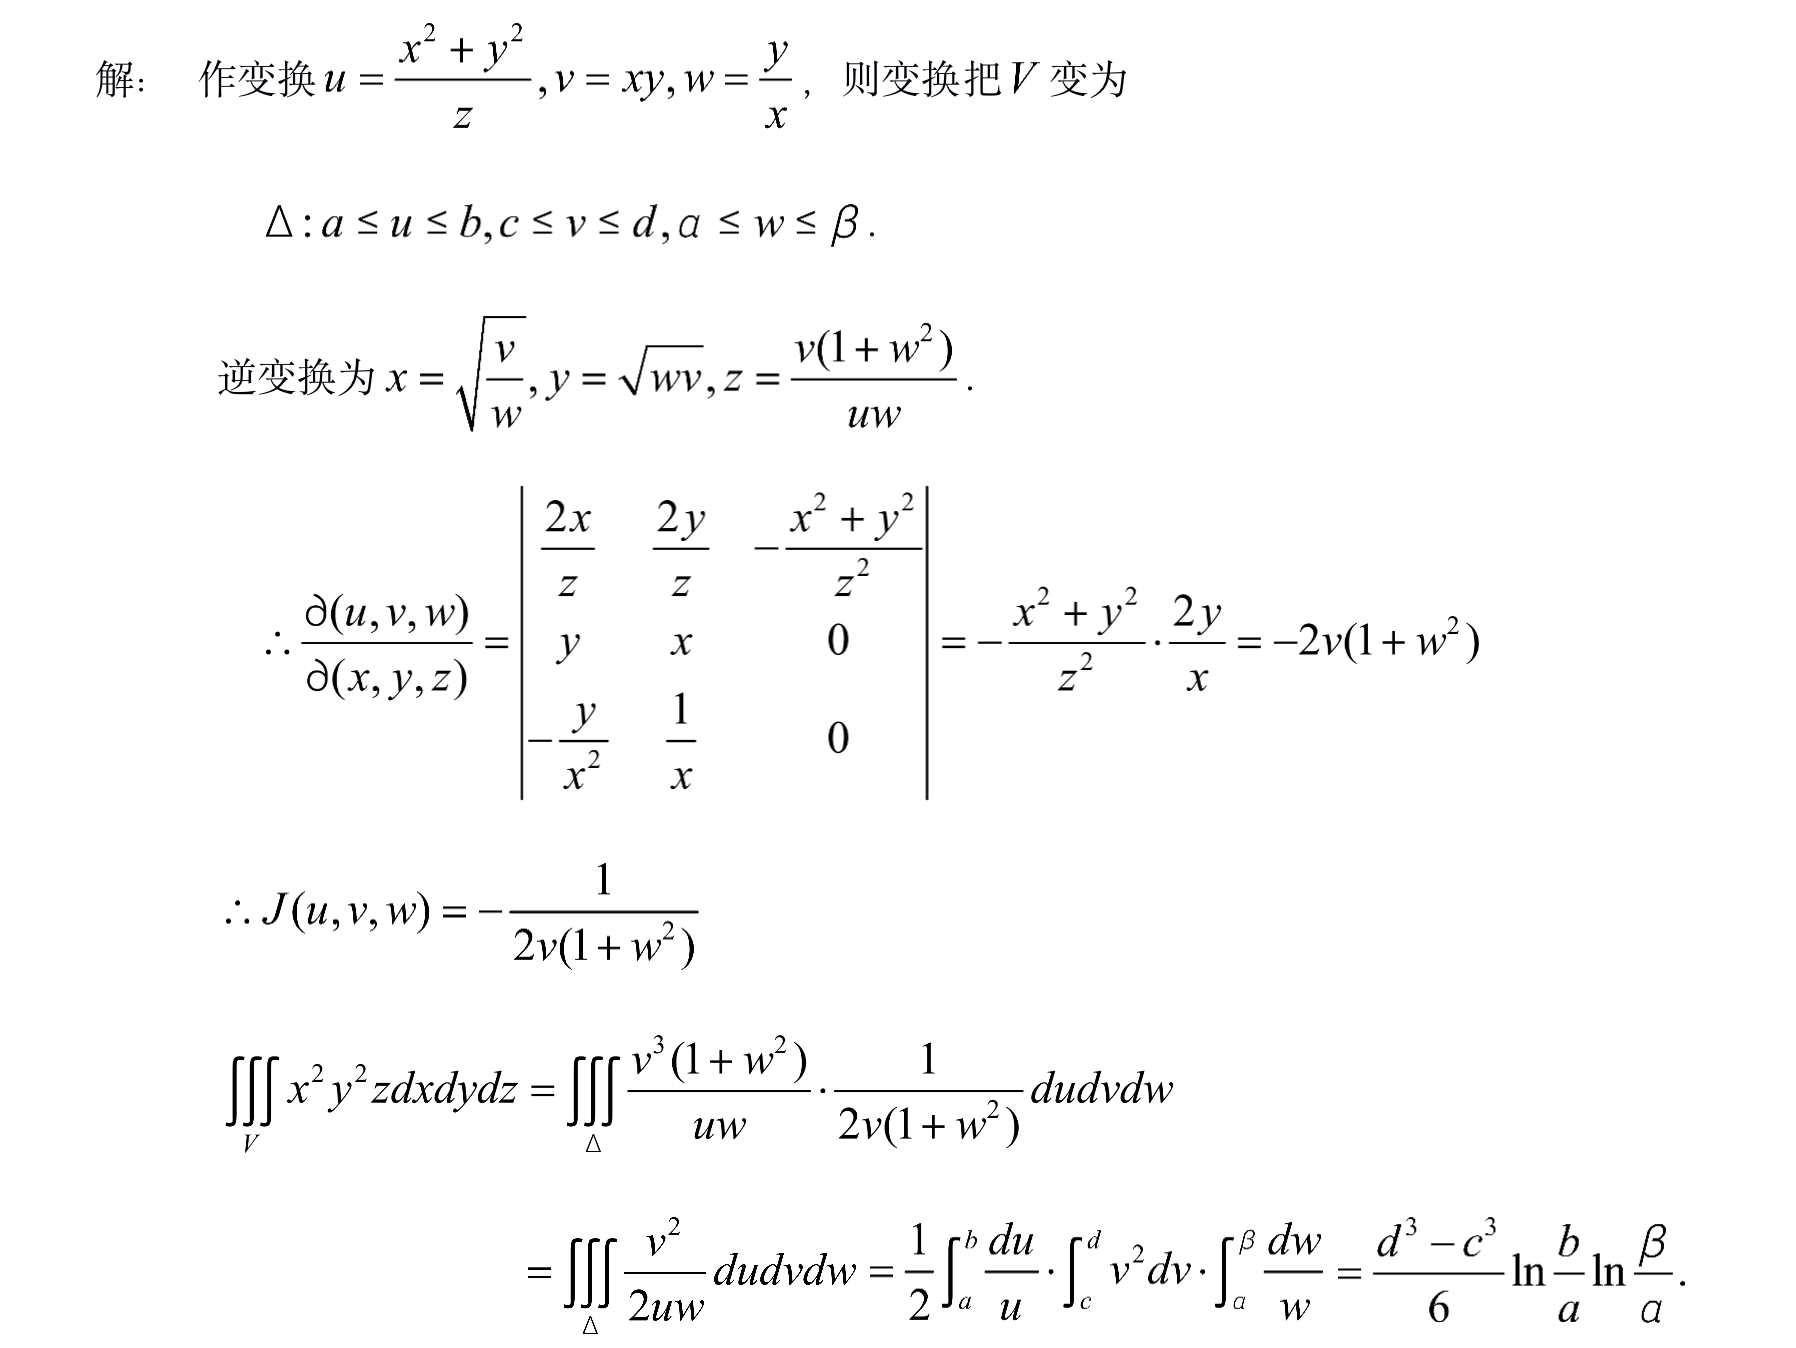
\includegraphics[width=1.0\textwidth]{img/f.jpg}
    \end{figure}
\end{frame} 

\begin{frame}
    \section{谢谢观看!}
\end{frame} 

\end{document}